\documentclass{uflamon}          % classe base para a monografia

%==============================================================================
% Utilizacao de pacotes
\usepackage[T1]{fontenc}         % usa fontes postscript com acentos
\usepackage[brazil]{babel}       % hifenização e títulos em português do Brasil
\usepackage[utf8]{inputenc}     % permite edição direta com acentos
\usepackage{amsmath}             % pacote da AMS para Matemática Avançada
\usepackage{amssymb}             % símbolos extras da AMS
\usepackage{latexsym}            % símbolos extras do LaTeX
\usepackage{graphicx}            % para inserção de gráficos
\usepackage{listings}            % para inserção de código
\usepackage{fancyvrb}            % para inserção de saídas de comandos
%\usepackage{enumerate}           % para personalizar lista enumeradas 
											%(incluso na classe)
\usepackage{longtable}           % para tambelas muito grandes NOVO!!!!

\usepackage{colortbl} % cores em tabelas
\newcolumntype{Z}{|>{\columncolor[gray]{0.9}}l|} %cor cinza em células
%\usepackage{array} % já incluso na classe
\newcolumntype{L}[1]{>{\raggedright\let\newline\\\arraybackslash\hspace{0pt}}m{#1}}
\newcolumntype{C}[1]{>{\centering\let\newline\\\arraybackslash\hspace{0pt}}m{#1}}
\newcolumntype{R}[1]{>{\raggedleft\let\newline\\\arraybackslash\hspace{0pt}}m{#1}}
\usepackage{multirow} % para juntar duas linhas em uma só

\usepackage{multicol} % para uso de várias colunas

% cores para os links cruzados
\usepackage{color}
\definecolor{rltred}{rgb}{0.2,0,0}
\definecolor{rltgreen}{rgb}{0,0.2,0}
\definecolor{rltblue}{rgb}{0,0,0.2}

\usepackage[colorlinks=true,
            urlcolor=rltblue,       % \href{...}{...} external (URL)
            filecolor=rltgreen,     % \href{...} local file
            linkcolor=rltred,       % \ref{...} and \pageref{...}
            citecolor=rltgreen,
            pdftitle={Exemplo de Uso da Classe Uflamon},
          pdfauthor={Joaquim Quinteiro Uchôa},
          pdfsubject={Este texto tem por objetivo servir de exemplo da classe Uflamon.},
          pdfkeywords={Comunicação Científica. 2. Pesquisa . 3. Pesquisa Científica. 
 					 4. Redação. 5. Monografia.}%
]{hyperref} % para referência cruzadas
%\usepackage{hyperref}            % para referência cruzadas
\usepackage{subfigure}           % figuras dentro de figuras
\usepackage{caption}            % remodelando o formato dos títulos de 
                                 % tabelas e figuras

% configuração padrão do listings   
\lstset{
   language=Java,
   extendedchars=true,
   tabsize=3,
   basicstyle=\footnotesize\ttfamily,
   stringstyle=\em,
   showstringspaces=false 
}

% para referências de acordo com a ABNT
% precisa instalar o abntex2 antes!!!
% http://abntex.codigolivre.org.br/
% comente se pretende usar outro padrão

%abnt-emphasize=bf coloca o título das bibliografias em negrito
%abnt-thesis-year=both
\usepackage[alf,abnt-etal-cite=3,abnt-etal-list=3,abnt-url-package=url,abnt-emphasize=bf]{abntex2cite}

% evite usar o hyperref com abntex, pode dar caca em urls... no linha anterior, informo
% para incluir urls usando o pacote url e não o hyperref
%
% caso queira o hyperref com abntex, comente a linha anterior e descomente a seguinte
%\usepackage[alf,abnt-etal-cite=3,abnt-etal-list=0,abnt-etal-text=emph]{abntex2cite}
%
% caso vc ainda use a versão anterior da abntex, comente a linha incluindo o abntex2cite
% e descomente a próxima linha 
%\usepackage[alf,abnt-etal-cite=3,abnt-etal-list=0,abnt-etal-text=emph]{abntcite}


% redefinindo formatação de títulos de tabelas e figuras


%==============================================================================
% para os fãs do Word, descomente as linhas abaixo
%\sloppy %mais espaço entre as linhas
%\usepackage{identfirst} %identando-se a primeira linha de cada seção
%\noindentfirst % Tire o comentário para manter o padrão do LaTeX.

%==============================================================================
% definido comandos na monografia - não é necessário na sua monografia 
% apenas para exemplificar a definição de novos comandos
\newcommand{\defs}[1]{\textsl{#1}}


% Especificando hifenizações que por ventura LaTeX não saiba fazer
% Por padrão 99,9% dos termos em português devem ser hifenizados corretamente.
\hyphenation{hardware software Li-nux am-bien-te diag-nos-ti-car coor-de-na-ção 
FAE-PE Recovery TelEduc Williams UFLA}

%==============================================================================
% Dados da monografia, capa: autor, titulo, banca, etc... - SUBSTITUA DE ACORDO
%==============================================================================
\author{Joaquim Quinteiro Uchôa}
\title{Uso da Classe Uflamon}
\subtitle{Exemplo para os Usuários}
\engtitle{Use of Uflamon Class}
\engsubtitle{Sample for Users}
\edicao{3$^a$ edição revista, atualizada e ampliada}
\date{2016}
\tipo{Tese apresentada à Universidade Federal de Lavras, como parte das exigências do Programa de Pós-Graduação em Monografia, área de concentração em TCC, para a obtenção do título de Doutor.}
% use \orientador ou \orientadora quando for o caso
\orientador{Prof. DSc. José Orientador}
%\orientadora{}
% use \coorientador ou \coorientadora quando for o caso
\coorientadora{Prof. DSc. Maria Orientadora } % comente se não tiver coorientador
%\coorientador{}
\local{Lavras -- MG}
\bancaum{Prof. MSc. Antônio Banca Um}{UFM}
\bancadois{Prof. DSc. João Banca Dois}{FCO} % comente se sua banca tiver só um professor
\bancatres{Profa. Esp. Eliza Banca Três}{BELMIS}
\bancaquatro{Prof. Esp. Carlos Banca Quatro}{IBGPLUS}
\defesa{30 de Fevereiro de 2016}
%==============================================================================
%##################################################
% Dados para Ficha catalográfica, gerada pelo sistema da Biblioteca da UFLA
% http://www.biblioteca.ufla.br/FichaCatalografica/
% dados para ficha catalográfica
% Elaboração da Ficha Catalográfica
\preparofichacat{Ficha catalográfica elaborada pela Coordenadoria de Processos Técnicos \\ da Biblioteca Universitária da UFLA}
% primeiro autor - como na primeira linha da ficha catalográfica
\fcautor{Uchôa, Joaquim Quinteiro}
% autores, separados por vírgula - na ficha catalográfica, no formato que
% vem após o título e a barra ("/")
\fcautores{Joaquim Quinteiro Uchôa}
% caso trabalho seja ilustrado (figuras, gráficos, tabelas, etc.), 
% então informar por meio do comando a seguir
% caso não seja ilustrado, basta comentá-lo
\fcilustrado{il.}
% dados da edição para a ficha 
\fcedicao{2$^a$ ed. rev., atual. e ampl.}
% tipo do trabalho (tese, dissertação, etc.), de acordo com sistema
% de geração de ficha catalográfica
\fctipo{Tese(doutorado)}
% ano da defesa, só precisa informar se for diferente do ano da publicação
% se forem iguais, comente a linha a seguir
\fcdatadefesa{2016}
% preencher aqui com os dados de catalogação gerados pelo sistema
\fccatalogacao{1. TCC. 2. Monografia. 3. Dissertação. 4. Tese. 5. Trabalho Científico – Normas. I. Universidade Federal de Lavras. II. Título.}
\fcclasi{808.066}

%##################################################

%\antesfichacat{\noindent Para citar este documento: \\UNIVERSIDADE FEDERAL DE LAVRAS. Biblioteca Universitária. \textbf{Manual de normalização e estrutura de trabalhos acadêmicos: TCC, monografias, dissertações e teses}. 2. ed. rev., atual. e ampl. Lavras, 2015. Disponível em: \url{http://www.biblioteca.ufla.br/wordpress/wpcontent/uploads/bdtd/manual_normalizacao_UFLA.pdf}. Acesso em: data de acesso.}

%\depoisfichacat{\noindent A reprodução e a divulgação total ou parcial deste trabalho são autorizadas, por qualquer meio convencional ou eletrônico, para fins de estudo e pesquisa, desde que citada a fonte.\\
%\newline
%{\small Este documento possui páginas em branco para facilitar a impressão frente-e-verso.}}

%##################################################

%##################################################

% para os exemplos do manual
%\newenvironment{exemplomanual}{
%\vspace{0.5cm}
%\noindent\begin{minipage}{\textwidth}
%\noindent\rule{\textwidth}{0.5pt}
%\vspace{-1cm}
%\begin{flushleft}
%}{
%\end{flushleft}
%\vspace{-0.6cm}
%\noindent\rule{\textwidth}{0.5pt}
%\vspace{0.3cm}
%\end{minipage}
%}

%\newenvironment{exemplomanuallista}{
%\vspace{0.3cm}
%\noindent\begin{minipage}{\textwidth - 0.5cm}
%\noindent\rule{\textwidth}{0.5pt}
%\vspace{-1cm}
%\begin{flushleft}
%}{
%\end{flushleft}
%\vspace{-0.6cm}
%\noindent\rule{\textwidth}{0.5pt}
%\vspace{0.3cm}
%\end{minipage}
%}

% por conta de alguns exemplos
%\usepackage{setspace}

%##################################################

% se vc já defendeu e tem o arquivo escaneado da folha de rosto, 
% descomente e altere o nome do arquivo
%\folhaAprovacaoAssinada{folharosto}

% Aqui começa o documento propriamente dito
\begin{document}

\maketitle

\dedic{Espaço reservado a dedicatória.}     % Dedicatórias\\

\thanks{Espaço reservado aos agradecimentos.}         % Agradecimentos

\epigrafe{ % citação opcional
Espaço reservado a epígrafe.\\
(Autor Desconhecido)}

% palavras-chave
\palchaves{Resumo. Palavras. Representativas.}
\resumo{O resumo deve conter palavras representativas do conteúdo do trabalho, localizadas abaixo do resumo, separadas por dois espaços, antecedidas da expressão palavras-chave. Essas palavras representativas são grafadas com a letra inicial em maiúscula, separadas entre si por ponto.}  % Resumo (digite aqui o resumo)

% keywords devem vir antes do abstract
\keywords{Summary. Words. Representative.} % keywords
\abstract{The abstract should contain representative words of the work content, located below the abstract, separated by two spaces, preceded by the keyword expression. These representative words are spelled with the first letter capitalized, separated by point.}

%##################################################

% Dados do guia
%\begin{titlepage}
%\pagestyle{empty}
%\renewcommand{\baselinestretch}{1}
%\enlargethispage{1.5cm}
%\input{reitoria}
%\cleardoublepage
%\end{titlepage}

%##################################################

% descomente para habilitar a lista desejada
\listoffigures                             % Lista de Figuras
%\listofilustracoes
%\listofgraficos							   % Lista de Gráficos
\listoftables                              % Lista de Tabelas
\listofquadros							   % Lista de Quadros
%\listofexemplos
%\listofteoremas
\tableofcontents                           % Sumário

\clearpage

\pagestyle{ufla}

%==============================================================================
% incluindo os capitulos
\chapter{\MakeUppercase{Introdução}}

O objetivo deste documento é apresentar o uso básico da classe \texttt{templufla} para a elaboração de trabalhos acadêmicos da \glsxtrfull{ufla}, utilizando a linguagem de marcação \LaTeX\ \cite[ p.17]{Lamport1994}. A maioria dos comandos (macros) e ambientes das classes básicas da linguagem é válida também nessa classe, que é estendida com comandos para confecção da capa, páginas de rosto, dedicatórias, etc. A classe atual foi baseada na classe \texttt{uflamon}, disponível em CC-BY 4.0, no site Overleaf.

Inicialmente, a classe \texttt{uflamon} foi criada de acordo com as normas da PRPG/UFLA para produção de TCC \cite{PRPG2006}. Essas normas foram posteriormente atualizadas, de maneira geral pela UFLA, para a produção de monografias, dissertações e teses \cite{BIB2010}. A classe \texttt{uflamon} foi mantida até a 2ª edição da normalização da \gls{ufla} \cite{UFLA:2015}.

Então, em 2025, com a publicação da 6ª edição da normalização \cite{UFLA:2025}, os atuais mantenedores criaram a classe \texttt{templufla} e o atual template, adaptando o antigo código para a nova norma, corrigindo inadequações, atualizando pacotes e ampliando o formato.

Este texto, com o objetivo de familiarizar o usuário da linguagem \LaTeX\ e demonstrar o uso da classe \texttt{templufla}, encontra-se organizado da seguinte maneira: 

A \autoref{sec:latex} apresenta conceitos básicos da linguagem \LaTeX, servindo como um ponto de início para novos usuários. 
A \autoref{sec:template} demonstra como utilizar os elementos da classe para a criação de trabalhos no formato da \gls{ufla}.
A \autoref{sec:listasEGlossario} é um tutorial básico de como usar os pacotes \texttt{glossaries} e \texttt{imakeidx} para criar listas, glossário e índice. 
A \autoref{sec:conclusao} apresenta comentários e observações finais.
Por fim, os Anexos \ref{anex:lorem1} e \ref{anex:lorem2} demonstram o uso dos anexos e o \autoref{apen:apendice} mostra como elaborar um apêndice simples.
\chapter{\MakeUppercase{Utilizando a Classe no Formato da UFLA}}\label{sec:template}

Agora que já temos o conhecimento básico sobre como a linguagem \LaTeX\ funciona, podemos nos aprofundar nos detalhes de como utilizar esse template (e, especialmente, a classe \texttt{templufla}) para gerar documentos padronizados de alta qualidade.

\section{Sobre as Seções (seção secundária)}\label{sec2:secoes}
\subsection{Sobre as Seções (seção terciária com texto extra comicamente grande para testar como será a quebra de linha do título)}\label{sec3:teste}
\subsubsection{Sobre as Seções (seção quaternária)}\label{sec4:teste}
\subsubsubsection{Sobre as Seções (seção quinária)}\label{sec5:teste}

Um dos fatores fundamentais no desenvolvimento de um trabalho acadêmico é sua organização. Na normalização da UFLA e da ABNT, os trabalhos podem ter formato de livro, como esse template, mas devem ser divididos em seções, não em capítulos e todo o texto pode ser dividido até a seção quinária.

No template, dispõem-se comandos para realizar tal divisão automaticamente, mas com uma importante observação: a seção primária utiliza o comando \verb|\chapter|. Isso foi feito para simplificar a migração de versões mais antigas e provavelmente será alterado no futuro. Abaixo estão listados os comandos de seccionamento disponíveis: 

\begin{alineas}
	\item \verb|\chapter|:  cria uma seção primária, que pode ser referenciada como \autoref{sec:template};
	\item \verb|\section|:  cria uma seção secundária, que pode ser referenciada como \autoref{sec2:secoes};
	\item \verb|\subsection|:  cria uma seção terciária, que pode ser referenciada como \autoref{sec3:teste};
	\item \verb|\subsubsection|:  cria uma seção quaternária, que pode ser referenciada como \autoref{sec4:teste};
	\item \verb|\subsubsubsection|:  cria uma seção quinária, que pode ser referenciada como \autoref{sec5:teste}.
\end{alineas}


\section{Alíneas e Subalíneas}
Segundo a normalização \cite{UFLA:2025}, ``as alíneas são usadas quando se deseja enumerar diversos assuntos de uma seção sem título próprio. Quando necessário, a alínea pode ser dividida em subalíneas.''

Nesse template, para listar elementos com alíneas, deve-se usar o ambiente \textbf{\texttt{alineas}}, que pode ser aninhado para criar subalíneas: 
\begin{lstlisting}[language={[LaTeX]TeX}]
	\begin{alineas}% [labelsep=0ex]
		\item item um;
		\item item dois:
		\begin{alineas} % subalíneas
			\item subitem 1;
			\item subitem 2.
		\end{alineas}
	\end{alineas}
\end{lstlisting}
Caso tenham letras duplicadas e queira mais espaço entre o indicador e o texto, basta adicionar a opção \texttt{[labelsep=0ex]} ao ambiente.

\vspace{18pt}
Abaixo é mostrado exemplo em texto retirado, na maior parte, do manual:
\begin{alineas}% adicione [labelsep=0ex] caso tenha letras duplicadas e queira mais espaço
	\item as alíneas são formadas pelos diversos assuntos que não possuem título próprio, dentro de uma mesma seção;
	\item o texto que antecede as alíneas termina em dois pontos;
	\item as alíneas devem ser indicadas alfabeticamente, em letra minúscula, seguida de parêntese. Utilizam-se letras dobradas, quando esgotadas as letras do alfabeto;
	\item as letras indicativas das alíneas devem apresentar recuo em relação à margem esquerda;
	\item o texto da alínea deve começar por letra minúscula e terminar em ponto e vírgula, exceto a última alínea que termina em ponto final;
	\item o texto da alínea deve terminar em dois pontos, se houver subalínea;
	\item a segunda e as seguintes linhas do texto da alínea começam sob a primeira letra do texto da própria alínea;
	\item sobre as subalíneas:
	\begin{alineas}
		\item as subalíneas devem começar por travessão seguido de espaço;
		\item as subalíneas devem apresentar recuo em relação à alínea;
		\item o texto da subalínea deve começar por letra minúscula e terminar em ponto e vírgula. A última subalínea deve terminar em ponto final, se não houver alínea subsequente;
		\item a segunda e as seguintes linhas do texto da subalínea começam sob a primeira letra do texto da própria subalínea;
		\item o recuo das margens também deve ser obedecido.
	\end{alineas}
\end{alineas}


\section{Figuras, Ilustrações e etc}

Utilizar figuras, ilustrações e elementos ``float'' no template é semelhante ao que foi explicado na \autoref{sec:latexFiguras}.
\begin{figure}[h]
	\centering
	\caption{Leão do site CTAN estudando \TeX}
	\label{fig:leaoCTAN}
	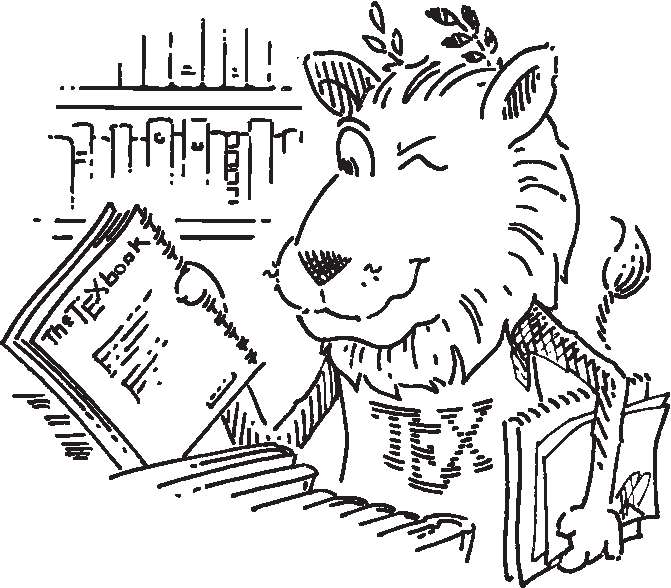
\includegraphics[width=0.6\textwidth]{imgs/ctanlion}
	\fonte{Duane Bibby, diponibilizado em \url{www.ctan.org/lion}}
\end{figure}


 Só é importante se atentar para dois detalhes: os títulos das figuras, que devem vir antes do \texttt{inludegraphics}, e a fonte, que deve ser posicionada após o \texttt{inludegraphics} e pode utilizar o comando pré definido \texttt{fonte}. Exemplo do código para a \autoref{fig:leaoCTAN}:
\begin{lstlisting}[language={[LaTeX]Tex}]
\begin{figure}
	\centering
	% \caption antes da figura
	\caption{Leão do site CTAN estudando \TeX} 
	\label{fig:leaoCTAN}
	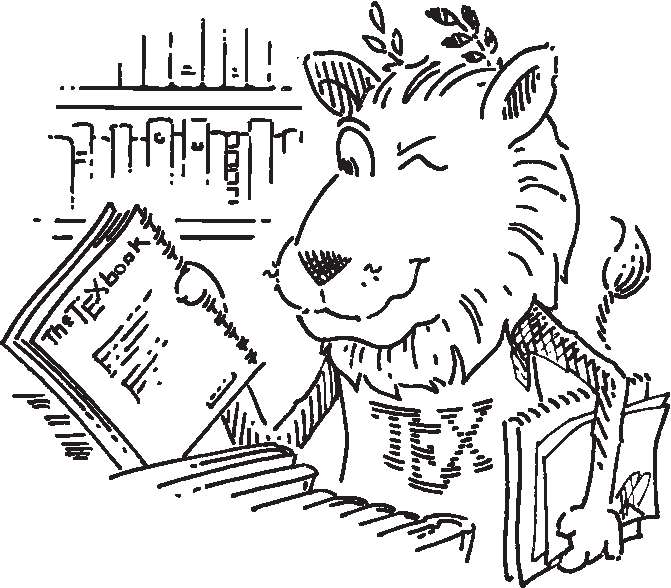
\includegraphics[width=0.6\textwidth]{imgs/ctanlion}
	\fonte{Duane Bibby, diponibilizador por \url{www.ctan.org}}
\end{figure}
\end{lstlisting}



\section{Quadros e Tabelas}\label{sec:tabelasUFLA}

A normalização da UFLA reconhece dois principais tipos de elementos tabulares, tabelas e quadros, com conteúdos e formatos específicos. 

\begin{table}[h]
	\centering
	\caption{Exemplo de Tabela} 
	\label{tab:exemplo2}
	\begin{tabular}{c c c c }
		\hline
		\linhadir{\bf Pessoa} & \linhadir{\bf Livros} & \linhadir{\bf Artigos} & \bf Palestras \\
		\hline
		$p_1$ & 1 & 3 & 4 \\
		$p_2$ & 1 & 3 & 3 \\
		$p_3$ & 1 & 3 & 4 \\
		$p_4$ & 3 & 5 & 2 \\
		\hline 
	\end{tabular}
	\vspace{0.3cm}
	\fonte{original} %Fonte do tabela
\end{table}

Tabelas envolvem principalmente números, utiliza-se linhas horizontais somente no topo, final e cabeçalhos, além disso utiliza-se linhas verticais somente nos cabeçalhos\footnote{Por isso a \autoref{tab:exemplo} não segue o padrão correto.}. Para reduzir o tamanho do código dos cabeçalhos, a classe \texttt{templufla} define do comando \texttt{linhadir}, que adiciona uma linha vertical à direita da célula. Abaixo mostra-se um exemplo do código para a \autoref{tab:exemplo2}:
\begin{lstlisting}[language={[LaTeX]Tex}]
\begin{table}[h]
	\centering
	\caption{Exemplo de Tabela} 
	\label{tab:exemplo2}
	\begin{tabular}{c c c c }
		\hline
		\linhadir{Pessoa}& \linhadir{Livros}& \linhadir{Artigos}& Palestras\\
		\hline
		$p_1$& 1& 3& 4\\
		$p_2$& 1& 3& 3\\
		$p_3$& 1& 3& 4\\
		$p_4$& 3& 5& 2\\
		\hline 
	\end{tabular}
	\vspace{0.3cm}
	\fonte{original} %Fonte do tabela
\end{table}
\end{lstlisting}


Quadros se diferem das tabelas por conterem principalmente dados textuais e suas células serem completamente fechadas. O \autoref{quad:exemplo} é um exemplo de quadro.

\begin{quadro}[h]
\centering
\caption{Opiniões sobre esse template}\label{quad:exemplo}
  \begin{tabular}{|l|p{9cm}|}
    \hline 
    \rowcolor[gray]{.9}
    \bf Nome& \bf Opinião\\
    \hline
    Jão& Desculpe, não posso comentar sobre isso.\\
    \hline
    Joana& Literalmente uma revolução do cinema nacional!\\
    \hline
    Jacquin& Esse autor é a vergonha da profisson!\\
    \hline
    Meu cachorro& Au! Au! Au! $\sim$Sons de papel sendo rasgado.\\
    \hline
    Overleaf& ASSINE, ASSINE O PREMIUM.\\
    \hline
    \end{tabular}
    
    \vspace{0.3cm}
	\fonte{original}
\end{quadro}


\section{Padrão das Referências}

Desde que o padrão descrito na \autoref{sec:Refs} seja seguido e partes importantes do template sejam mantidas, as referências não devem ser um problema. O template já vem configurado para o formato padrão da ABNT, desde que os arquivos \texttt{abntex.*}, o preâmbulo e a chamada dos comandos \texttt{bibliographystyle}, \texttt{citeoption}, \texttt{refencias} e \texttt{bibliography}, próximos ao final do arquivo principal, sejam mantidos.

É comum referências serem um problema e, apesar do \LaTeX\ ajudar muito nisso, o processo ainda pode ser complicado. O pacote \texttt{abntex2} está desatualizado, as correções precisaram ser \emph{hard-coded} e o arquivo principal reflete isso.

\textbf{Então, se você quer que as citações e referências sejam tão simples quanto adicionar um \texttt{bibtex} e usar o comando \texttt{cite}, EU TE SUPLICO, não altere o preâmbulo nem os comandos relacionados às referências no \texttt{tempulfa\_main.tex}.}

Referências sortidas para contribuir para a lista ao final (ignore): \cite{Eco1996,Booth2000,BIB2010,Hexsel2004,Franca2001,Gil2002,Porto2002,Silva2005,UFLA:2015,Moura1998,NBR6023:2002,LeGuin:1987}


\chapter{\MakeUppercase{Conclusão}}\label{sec:conclusao}

O objetivo deste documento foi apresentar o uso básico da classe \texttt{templufla} para a elaboração de trabalhos acadêmicos da UFLA utilizando \LaTeX. Após edição em \LaTeX, o usuário pode gerar arquivos PDF \cite{PDF2004} ou PostScript \cite{PostScript1999} com grande facilidade.



%==============================================================================
% Incluindo bibliografia
%\bibliographystyle{plain}             % estilo para labels em numeros
%\bibliographystyle{alpha}             % estilo para labels em iniciais
\bibliographystyle{abntex2-alf}           % estilo para referências usando ABNT, 
                                       % precisa instalar o abntex para usar!!!

%inclui Referências Bibliográficas
%inclui Referências Bibliográficas
\referencias
\bibliography{refbib}			% arquivo exemplo refbib.bib
%==============================================================================
% Incluindo anexos num1erados com letras maiusculas.
%\apendices
\apendice{O que são apêndices}
\label{cap:apendice}

Um apêndice é um suporte elucidativo e ilustrativo do texto principal. Sua função é agrupar elementos que são úteis à compreensão do texto e que, no entanto, podem ser apresentados à parte sem prejuízo à compreensão. É útil para a apresentação de modelagens, diagramas extensos, listagens de código-fonte de programas e demais elementos que o autor julgar necessário à complementação do tema abordado no texto principal.


%==============================================================================
% Fim do texto
\end{document}
